\section{Environmental Conditions}
The experiment was carried out between the 11th of November 2018 \& the 18th of November 2018. It was typically carried out between the hours of 18:00 \& 00:00. We collected this data during the winter time as the night sky emerges earlier in the evening. This experiment was carried out during the Moon's waxing crescent phase. This was done in order to avoid sky glow from the Moon artificially increasing the photopollution of the town. There was a little precipitation when we collected data from the town of Tipperary, however, the weather cleared up thereafter. It was important that this experiment was carried out in November rather then December, as the Christmas lights put up during the latter period would have also artificially increased the photopollution value. 

\section{Apparatus Used} 
\begin{itemize}
\item Celestron Astromaster 102AZ  with an aperture of 102 mm with 20 mm telescope eyepiece lens.\cite{telescope}
\item Smartphone with photometer app preinstalled (LUX Light Metre Pro).\cite{photometer}
\item Purple Toshiba Laptop running Ubuntu with the latest version of Python 2.7 installed. Python modules we utilised include: Pandas, Scipy, Numpy, and Mathplotlib. We used Python primarily for data analysis during this project.\cite{purple_toshiba}\cite{python}\cite{scipy}
\item QGIS for generating a photopollution map, and population density heat map.\cite{QGIS_software}
\item Renault Clio car used for traveling to all the great sites of Munster.\cite{fab}
\end{itemize}

\section{Labelled Diagram}
\begin{figure}[H]
    \centering
    \begin{subfigure}{.48\textwidth}
        \centering
        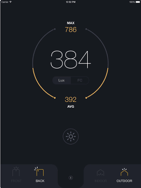
\includegraphics[width=\textwidth]{photometer}
        \caption{Photometer/LUX Light Metre}
    \end{subfigure}
    \hfill
    \begin{subfigure}{.48\textwidth}
        \centering
        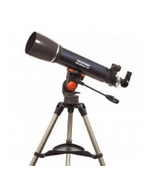
\includegraphics[width=\textwidth]{telescope}
        \caption{Telescope}
    \end{subfigure}
\end{figure}

\section{Procedure}  
\begin{enumerate}
\subsection{Data Collection}
\item We placed the telescope as close to the centre of the town as physically possible. (We used the same telescope eyepiece lens, photometer app and telescope throughout the experiment)
\item Once the telescope was set up, we placed the smartphone’s lens on the eyepiece lens of the telescope. We then opened the smartphone photometer application and prepared for recording the data.
\item We recorded our measurements with the telescope pointing towards zenith. This value is the photopollution produced by this particular area. We also recorded a maximum and minimum LUX value from that same portion of the sky.
\item We repeated Steps 1 - 4 at 20 different locations. We traveled to these sites using the fantastic Renault Clio, and included all the counties of Munster in this project.
\subsection{Data Analysis and Outcomes}
\item Once we collected all the data, it was time to find out whether there was a correlation between photopollution and population density. First, we visited the Central Statistics Office's website and downloaded a file containing the population density data for all the sites that we gathered data from.
\item Once we acquired this data, we inputted all the photopollution values collected using our photometer application into a Solver python program that Conor developed. This program printed all values inputted into it, found a correlation between the two variables, printed the correlation coefficient, standard deviation, and the equation describing the correlation. It also printed the correlation coefficient of Walker's Law, and outputted all the graphs that can be found throughout this Project Book. This was done using Mathpoltlib. (The code can be found in Appendices.)
\item Using this model, we were able to develop a grading system that can determine what any photopollution value produced in any particular area would mean in relation to the stargazing conditions. We did this by setting Limerick City as the baseline for terrible stargazing conditions (We choose Limerick City as, it was the site with the lowest population density that we deemed to be characterised with terrible stargazing conditions), and using this baseline we extrapolated five different grades for stargazing conditions, from excellent to terrible.  
\item Using the mathematical model and grading system, we generated a photopollution map using the software QGIS, and compared it against a nighttime survey of Ireland provided by the VIIRS 2018 (March) Radiance. 
\item Following which, Conor developed another Python program, and an app which incorporates our mathematical model and grading system to show the potential practical appliciations. This grading system took Limerick City as the base point for terrible stargazing conditions and giving a total of five different grades including terrible. (Code can be found in Appendices.)
\end{enumerate}




